% Siconos-Doc version 1.3.0, Copyright INRIA 2005-2006.
% Siconos is a program dedicated to modeling, simulation and control
% of non smooth dynamical systems.	
% Siconos is a free software; you can redistribute it and/or modify
% it under the terms of the GNU General Public License as published by
% the Free Software Foundation; either version 2 of the License, or
% (at your option) any later version.
% Siconos is distributed in the hope that it will be useful,
% but WITHOUT ANY WARRANTY; without even the implied warranty of
% MERCHANTABILITY or FITNESS FOR A PARTICULAR PURPOSE.  See the
% GNU General Public License for more details.
%
% You should have received a copy of the GNU General Public License
% along with Siconos; if not, write to the Free Software
% Foundation, Inc., 51 Franklin St, Fifth Floor, Boston, MA  02110-1301  USA
%
% Contact: Vincent ACARY vincent.acary@inrialpes.fr 
%/
\documentclass[10pt]{article}
%$Id: macro.tex,v 1.10 2004/12/08 13:38:58 acary Exp $


%\usepackage{a4wide}
\textheight 25cm
\textwidth 16.5cm
\topmargin -1cm
%\evensidemargin 0cm
\oddsidemargin 0cm
\evensidemargin0cm
\usepackage{layout}


\usepackage{amsmath}
\usepackage{amssymb}
\usepackage{minitoc}
%\usepackage{glosstex}
\usepackage{colortbl}
\usepackage{hhline}
\usepackage{longtable}

%\usepackage{glosstex}
%\def\glossaryname{Glossary of Notation}
\def\listacronymname{Acronyms}

\usepackage[outerbars]{changebar}\setcounter{changebargrey}{20}
%\glxitemorderdefault{acr}{l}

%\usepackage{color}
\usepackage{graphicx,epsfig}
\graphicspath{{figure/}}
\usepackage[T1]{fontenc}
\usepackage{rotating}

%\usepackage{algorithmic}
%\usepackage{algorithm}
\usepackage{ntheorem}
\usepackage{natbib}


%\renewcommand{\baselinestretch}{2.0}
\setcounter{tocdepth}{2}     % Dans la table des matieres
\setcounter{secnumdepth}{3}  % Avec un numero.



\newtheorem{definition}{Definition}
\newtheorem{lemma}{Lemma}
\newtheorem{claim}{Claim}
\newtheorem{remark}{Remark}
\newtheorem{assumption}{Assumption}
\newtheorem{example}{Example}
\newtheorem{conjecture}{Conjecture}
\newtheorem{corollary}{Corollary}
\newtheorem{OP}{OP}
\newtheorem{problem}{Problem}
\newtheorem{theorem}{Theorem}


\newcommand{\CC}{\mbox{\rm $~\vrule height6.6pt width0.5pt depth0.25pt\!\!$C}}
\newcommand{\ZZ}{\mbox{\rm \lower0.3pt\hbox{$\angle\!\!\!$}Z}}
\newcommand{\RR}{\mbox{\rm $I\!\!R$}}
\newcommand{\NN}{\mbox{\rm $I\!\!N$}}

\newcommand{\Mnn}{\mathcal M^{n\times n}}
\newcommand{\Mnp}[2]{\ensuremath{\mathcal M^{#1\times #2}}}



\newcommand{\Frac}[2]{\displaystyle \frac{#1}{#2}}

\newcommand{\DP}[2]{\displaystyle \frac{\partial {#1}}{\partial {#2}}}

% c++ variables writting
\newcommand{\varcpp}[1]{\textit{#1}}
% itemize
\newcommand{\bei}{\begin{itemize}}
\newcommand{\ei}{\end{itemize}}

\newcommand{\ie}{i.e.}
\newcommand{\eg}{e.g.}
\newcommand{\cf}{c.f.}
\newcommand{\putidx}[1]{\index{#1}\textit{#1}}

\def\Er{{\rm I\! R}}
\def\En{{\rm I\! N}} 
\def\Ec{{\rm I\! C}}
 
\def\zc{\hat{z}}
\def\wc{\hat{w}}

\font\tete=cmr8 at 8 pt
\font\titre= cmr12 at 20 pt 
\font\titregras=cmbx12 at 20 pt

%----------------------------------------------------------------------
%                  Modification des subsubsections
%----------------------------------------------------------------------
\makeatletter
\renewcommand\thesubsubsection{\thesubsection.\@alph\c@subsubsection}
\makeatother

%----------------------------------------------------------------------
%             Redaction note environnement
%----------------------------------------------------------------------
\makeatletter
\theoremheaderfont{\scshape}
\theoremstyle{marginbreak}
\theorembodyfont{\upshape}
%\newtheorem{rque}{\bf Remarque}[chapter]
%\newtheorem{rque1}{\bf \fsc{Remarque}}[chapter] !!! \fsc est une commande french
\newtheorem{ndr1}{\textbf{\textsc{Redaction note}}}[section]

\newenvironment{ndr}%
{%
\tt
%\centerline{---oOo---}
\noindent\begin{ndr1}%
}%
{%
\begin{flushright}%
%\vspace{-1.5em}\ding{111}
\end{flushright}%
\end{ndr1}%
%\centerline{---oOo---}
}

\makeatother

%----------------------------------------------------------------------
%             Redaction note environnement V.ACARY
%----------------------------------------------------------------------
\makeatletter
\theoremheaderfont{\scshape}
\theoremstyle{marginbreak}
\theorembodyfont{\upshape}
%\newtheorem{rque}{\bf Remarque}[chapter]
%\newtheorem{rque1}{\bf \fsc{Remarque}}[chapter] !!! \fsc est une commande french
\newtheorem{ndr1va}{\textbf{\textsc{Redaction note V. ACARY}}}[section]

\newenvironment{ndrva}%
{%
\tt
%\centerline{---oOo---}
\noindent\begin{ndr1va}%
}%
{%
\begin{flushright}%
%\vspace{-1.5em}\ding{111}
\end{flushright}%
\end{ndr1va}%
%\centerline{---oOo---}
}

\makeatother
%----------------------------------------------------------------------
%             Redaction note environnement V.ACARY
%----------------------------------------------------------------------
\makeatletter
\theoremheaderfont{\scshape}
\theoremstyle{marginbreak}
\theorembodyfont{\upshape}
%\newtheorem{rque}{\bf Remarque}[chapter]
%\newtheorem{rque1}{\bf \fsc{Remarque}}[chapter] !!! \fsc est une commande french
\newtheorem{ndr1fp}{\textbf{\textsc{Redaction note F. PERIGNON}}}[section]

\newenvironment{ndrfp}%
{%
\tt
%\centerline{---oOo---}
\noindent\begin{ndr1fp}%
}%
{%
\begin{flushright}%
%\vspace{-1.5em}\ding{111}
\end{flushright}%
\end{ndr1fp}%
%\centerline{---oOo---}
}

\makeatother
%----------------------------------------------------------------------
%                  Chapter head enviroment
%----------------------------------------------------------------------
\newenvironment{chapter_head}
{%
\begin{center}%
-------------------- oOo --------------------\\%
\ \\%
\begin{minipage}[]{14cm}%
\noindent\normalsize\advance\baselineskip-1pt %
}%
{%
\par\end{minipage}%
\ \\%
\ \\%
-------------------- oOo --------------------
\end{center}%
\vspace*{\stretch{1}}%
\clearpage%
\thispagestyle{empty}%
\vspace*{\stretch{1}}%
\minitoc%
\vspace*{\stretch{2}}%
\clearpage%
}

%%% Local Variables: 
%%% mode: latex
%%% TeX-master: "report"
%%% End: 

\usepackage{psfrag}
\usepackage{fancyhdr}
\usepackage{subfigure}
%\renewcommand{\baselinestretch}{1.2}
\textheight 23cm
\textwidth 16cm
\topmargin 0cm
%\evensidemargin 0cm
\oddsidemargin 0cm
\evensidemargin 0cm
\usepackage{layout}
\usepackage{mathpple}
\usepackage[T1]{fontenc}
%\usepackage{array}
\makeatletter
\renewcommand\bibsection{\paragraph{References
     \@mkboth{\MakeUppercase{\bibname}}{\MakeUppercase{\bibname}}}}
\makeatother
%% style des entetes et des pieds de page
\fancyhf{} % nettoie le entetes et les pieds
\fancyhead[L]{}
\fancyhead[R]{\thepage}
\fancyfoot[C]{}%
\begin{document}
\thispagestyle{empty}
\title{Dynamical Systems formulations in Siconos.}
\author{F. P\'erignon}

\date{For Kernel version 1.3.0 \\
 \today}
\maketitle

\pagestyle{fancy}

\section{Class Diagram}
There are five possible formulations for dynamical systems in Siconos,
three for first order systems and two for second order Lagrangian systems. The main class is DynamicalSystem, all other derived from this one, as shown in the following diagram:
\begin{figure}[htbp]
  \centering
 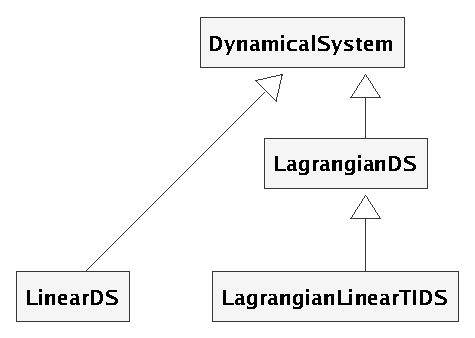
\includegraphics[width=0.3\textwidth]{./DSClassDiagram.eps}
  \label{DSDiagram}
\end{figure}
% DYNAMICAL SYSTEMS
\section{General non linear first order dynamical systems \\ $\rightarrow$ class \it{DynamicalSystem}}
This is the top class for dynamical systems. All other systems classes are derived from this one. \\

A general dynamical systems is described by the following set of $n$ equations, completed with initial conditions:
\begin{eqnarray} \label{firstOrderSystem}
  \dot x &=& f(x,t) + T(x) u(x, t) + r \\
  x(t_0)&=&x_0 
\end{eqnarray}

\begin{itemize}
\item $x$: state of the system - Vector of size $n$.
\item $f(x,t)$: sometimes called vector field - Vector of size $n$.
\item $u(x, t)$: control term - Vector of size $uSize$.
\item $T(x)$: $n\times uSize$ matrix, related to control term.
\item $r$: input due to non-smooth behavior - Vector of size $n$.
\end{itemize}

The Jacobian matrix, $\nabla_x f(x,t)$, of $f$ according to $x$, $n\times n$ square matrix, is also a member of the class. \\

Initial conditions are given by the member $x_0$, vector of size $n$. This corresponds to x value when
simulation is starting, ie after a call to strategy->initialize(). \\

There are plug-in functions in this class for $f$, its Jacobian, $jacobianXF$, $u$ and $T$. All
of them can handle a vector of user-defined parameters:

\textbf{Required parameters:} $n$, $x0$, $f$ (as a plug-in), its Jacobian.

\textbf{Main functions of the class:}
\begin{itemize}
\item \textit{computeRhs(time)}: to compute right hand side of equation \eqref{firstOrderSystem} (saved in member rhs)
\item \textit{computeJacobianXRhs(time)}: to compute the Jacobian according to x of the right-hand side.
\item \textit{computeF(time)}: to compute $f(x,t)$ and save it into rhs member. Plug-in function must be set with \it{setComputeFFunction(pluginPath, functionName)}. 
\item \textit{computeJacobianXF(time)}: to compute $\nabla_x f(x,t)$, and save it into member JacobianXF. Plug-in function must be set with \textit{setComputeJacobianXFFunction(pluginPath, functionName)}.
\end{itemize}
With \textit{pluginPath} the name of the library that contains your plugin and functionName the name you give to the function. 
(for example if you defined your plug-in for f in the file MyPlugin.cpp and call the function computeMyF, then pluginPath ="MyPlugin.so" and functionName = "computeMyF".)
Warning: the name of the plugin file must end with the string "Plugin", and the length of the string before "Plugin" must not exceed 6 letters. \\
The signature of each function (ie the number and type of arguments) must be exactly the same as the one given in Kernel/src/plugin/DefaultPlugin.cpp for the corresponding function. 

% LINEAR DS
\section{First order linear dynamical systems $\rightarrow$ class \textit{LinearDS}}

Derived from DynamicalSystem, described by the set of $n$ equations and initial conditions: 
\begin{eqnarray}
  \dot x &=& A(t)x(t)+Tu(t)+b(t)+r \\
  x(t_0)&=&x_0 
\end{eqnarray}
With:
\begin{itemize}
\item $A(t)$: $n\times n$ matrix, state independent but possibly time-dependent.
\item $b(t)$: Vector of size $n$, possibly time-dependent.
\end{itemize}
Other variables are those of DynamicalSystem class. \\
$A$ and $B$ have corresponding plug-in functions. \\

Links with vectorField and its Jacobian are: 
\begin{eqnarray}
  f(x,t) &=& A(t)x(t)+b(t) \\
  jacobianXF&=&\nabla_x f(x,t) = A(t) 
\end{eqnarray}

Main functions of the class:
\begin{itemize}
\item \textit{computeRhs(time)}: to compute $Ax+b+Tu$ (saved in member rhs)
\item \textit{computeJacobianXRhs(time)}: compute $A(t)$.
\item \textit{computeA(time)}: to compute $A(t)$. Plug-in function must be set with \textit{setComputeAFunction(pluginPath, functionName)}. 
\item \textit{computeB(time)}: to compute $b(t)$. Plug-in function must be set with \textit{setComputeBFunction(pluginPath, functionName)}.
\end{itemize}

% LINEAR TIDS
\section{First order time-invariant linear dynamical systems $\rightarrow$ class \textit{LinearTIDS}}

Derived from DynamicalSystem, described by the set of $n$ equations and initial conditions: 
\begin{eqnarray}
  \dot x &=& Ax(t)+Tu(t)+b+r \\
  x(t_0)&=&x_0 
\end{eqnarray}
With:
\begin{itemize}
\item $A(t)$: $n\times n$ constant matrix
\item $b(t)$: constant vector of size $n$
\end{itemize}
Other variables are those of DynamicalSystem class. \\

Links with vectorField and its Jacobian are: 
\begin{eqnarray}
  f(x,t) &=& Ax(t)+b \\
  jacobianXF&=&\nabla_x f(x,t) = A
\end{eqnarray}

Main functions of the class:
\begin{itemize}
\item \textit{computeRhs(time)}: to compute $Ax+b+Tu$ (saved in member rhs)
\item \textit{computeJacobianXRhs(time)}: compute $A(t)$.
\end{itemize}

% LAGRANGIANDS
\section{Second order non linear Lagrangian dynamical systems \\  $\rightarrow$ class \textit{LagrangianDS}}

Lagrangian second order non linear systems are described by the following set of $nDof$ equations + initial conditions:
\begin{eqnarray}
 M(q) \ddot q + NNL(\dot q, q) + F_{Int}(\dot q , q , t) &=& F_{Ext}(t) + p \\
 q(t_0) &=& q0 \\
 \dot q(t_0) &=& velocity0 
\end{eqnarray}
With:
\begin{itemize}
\item $M(q)$: $nDof\times nDof$ matrix of inertia.
\item $q$: state of the system - Vector of size $nDof$.
\item $\dot q$ or $velocity$: derivative of the state according to time - Vector of size $nDof$.
\item $NNL(\dot q, q)$:  non linear terms, time-independent - Vector of size $nDof$.
\item $F_{Int}(\dot q , q , t)$: time-dependent linear terms - Vector of size $nDof$.
\item $F_{Ext}(t)$: external forces, time-dependent BUT do not depend on state - Vector of size $nDof$.
\item $p$: input due to non-smooth behavior - Vector of size $nDof$.
\end{itemize}

The following Jacobian are also member of this class:
\begin{itemize}
\item jacobianQFInt = $\nabla_q F_{Int}(t,q,\dot q)$ - $nDof\times nDof$ matrix.
\item jacobianVelocityFInt = $\nabla_{\dot q} F_{Int}(t,q,\dot q)$ - $nDof\times nDof$ matrix.
\item jacobianQNNL = $\nabla_q NNL(q,\dot q)$ - $nDof\times nDof$ matrix.
\item jacobianVelocityNNL = $\nabla_{\dot q}NNL(q,\dot q)$ - $nDof\times nDof$ matrix.
\end{itemize}


There are plug-in functions in this class for $F_{int}$, $F_{Ext}$, $M$, $NNL$ and the four Jacobian matrices. All
of them can handle a vector of user-defined parameters. \\
Call \textit{computeOperator(...)} to compute value for operator = {$FInt$, $FExt$, $Mass$, $NNL$, $JacobianQFInt$, $JacobianVelocityFInt$, $JacobianQNNL$,$JacobianVelocityNNL$}. For any of them, link with plug-in function must be set using \textit{setComputeOperatorFunction(pluginPath,pluginName)}.

Links with first order dynamical system are: 
\begin{eqnarray}
  n &= &2nDof \\
  x &=&\left[\begin{array}{c}q \\ \dot q \end{array}\right] \\
  f(x,t) &=&  \left[\begin{array}{c} \dot q \\ M^{-1}(F_{Ext}-F_{Int}-NNL) \end{array}\right] \\
  \\
  \nabla_x f(x,t) &=& 
  \left[\begin{array}{cc} 
      0_{nDof\times nDof} & I_{nDof\times nDof} \\
      \nabla_q(M^{-1})(F_{Ext}-F_{Int}-NNL) -M^{-1}\nabla_q(F_{Int}+NNL) &  -M^{-1}\nabla_{\dot q}(F_{Int}+NNL) 
    \end{array}\right] \\
  r &=& \left[\begin{array}{c} 0_{nDof} \\ p \end{array}\right] \\
  u(x,\dot x,t) &=& u_L(\dot q, q, t) \text{  (not yet implemented)} \\
  T(x) &=& \left[\begin{array}{c} 0_{nDof} \\ T_L(q) \end{array}\right] \text{  (not yet implemented)} \\
\end{eqnarray}
With $0_{n}$ a vector of zero of size $n$, $0_{n\times m}$ a $n\times m$ zero matrix and
$I_{n\times n}$, identity $n\times n$ matrix. \\

Warning: control terms ($Tu$) are not fully implemented in Lagrangian systems. This will be part of future version.

% LAGRANGIAN LINEAR TIME INVARIANT DS
\section{Second order linear and time-invariant Lagrangian dynamical systems $\rightarrow$ class \textit{LagrangianLinearTIDS}}

\begin{eqnarray}
M \ddot q + C \dot q + K q =  F_{Ext}(t) + p
\end{eqnarray}

With:
\begin{itemize}
\item $C$: constant viscosity $nDof\times nDof$ matrix 
\item $K$: constant rigidity $nDof\times nDof$ matrix 
\end{itemize}

And: 
\begin{eqnarray}
F_{Int} &=& C \dot q + K q \\
NNL &=& 0_{nDof} 
\end{eqnarray}

\section{How to handle parameters in plug-in functions for Dynamical Systems}

\subsection{User management}

All plug-in in DynamicalSystem class, or in its derived classes, have a possible user-defined parameter argument, 
usually the last one in the list (see DefaultPlugin.cpp file). This argument consists in a pointer to SimpleVector, 
which can be defined by user in the following way: \\
In the main input file of your sample (python or cpp), 
\begin{itemize}
\item first declare and define a SimpleVector
\item assign this SimpleVector to the DynamicalSystem plug-in, using one of the two following:
\begin{itemize}
\item $setParameter(yourVector, "id")$, where $"id"$ is the plug-in name (see table \ref{parametersIdList} below for the list of available ids for each class). In that case, yourVector is a SimpleVector (not a pointer!).
This will set yourVector values as an input list for parameters in plug-in function $"id"$. 
\item  $setParameterPtr(yourVector, "id")$, where $"id"$ is the plug-in name (see table \ref{parametersIdList} below for the list of available ids for each class). Here, yourVector is a pointer to SimpleVector. 
This will link parameters vector in plug-in function $"id"$ to yourVector. (Warning: this means  that any change to one of them (yourVector and parameter) will affect the other). 
\end{itemize}
\item then in the corresponding yourPlugin.cpp file, the variable $param$ corresponds to the vector you defined. 
\end{itemize}

Example: suppose that you defined a LagrangianDS named lds, and want to set two parameters in the external forces, say $mu$ and $lambda$. Then cpp input file looks like: \\
\expandafter\ifx\csname indentation\endcsname\relax%
\newlength{\indentation}\fi
\setlength{\indentation}{0.5em}
\begin{flushleft}
{$//$\textit{} In the main file:{}\mbox{}\\
}\mbox{}\\
{\bf double} mu;\mbox{}\\
{\bf double} lambda; \mbox{}\\
\mbox{}\\
{$//$\textit{} ... give mu and lambda the required value{}\mbox{}\\
}{$//$\it{} ... declare and built your dynamical system{}\mbox{}\\
}DynamicalSystem $\ast$ lds = {\bf new} LagrangianDS($\ldots$) \mbox{}\\
{$//$\it{} $=$$=$$=$ First way, with setParameter function $=$$=$$=$ {}\mbox{}\\
}{$//$\it{} declare and built a SimpleVector of size 2{}\mbox{}\\
}SimpleVector parameters(2);\mbox{}\\
parameters(0) = mu;\mbox{}\\
parameters(1) = lambda;\mbox{}\\
\mbox{}\\
lds$\rightarrow$setParameter(parameters,{\tt"fExt"});\mbox{}\\
\mbox{}\\
{$//$\it{} In this case, if parameters values are change after this step, this won´t affect param values inside the dynamical system. {}\mbox{}\\
}\mbox{}\\
{$//$\it{} $=$$=$$=$ Second way, with setParameterPtr function $=$$=$$=$ {}\mbox{}\\
}{$//$\it{} declare and built a pointer to SimpleVector of size 2{}\mbox{}\\
}SimpleVector $\ast$ parameters = {\bf new} SimpleVector(2);\mbox{}\\
($\ast$parameters)(0) = mu;\mbox{}\\
($\ast$parameters)(1) = lambda;\mbox{}\\
\mbox{}\\
lds$\rightarrow$setParameter(parameters,{\tt"fExt"});\mbox{}\\
\mbox{}\\
{$//$\it{} Warning: in that case, from this point any change in parameters will affect param value in the dynamical system.{}\mbox{}\\
}{$//$\it{} {}\mbox{}\\
}\mbox{}\\
{$//$\it{} Then in the plug-in file, you have access to the parameter values: {}\mbox{}\\
}\mbox{}\\
{\bf extern} {\tt"C"} {\bf void} computeFExt({\bf const} {\bf unsigned} {\bf int}\&sizeOfq, {\bf const} {\bf double} $\ast$time, {\bf double} $\ast$fExt, {\bf double} $\ast$param)\mbox{}\\
\{\mbox{}\\
\hspace*{2\indentation}{\bf for}({\bf unsigned} {\bf int} i =0; i$<$sizeOfq;++i)\mbox{}\\
\hspace*{4\indentation}fExt[i] = cos(param[1]$\ast$time) + param[0] ;\mbox{}\\
\mbox{}\\
\hspace*{2\indentation}{$//$\it{} this means that Fext $=$ cos(lambda t) $+$ mu {}\mbox{}\\
}\mbox{}\\
\}\mbox{}\\
\mbox{}\\
\mbox{}\\
\end{flushleft}

Warning: there is no relation between the name you give to your plug-in function (computeFExt in previous example) and the 
name given when you call $setParameter(..., id)$ ($"Fext"$ in previous example). 

\subsection{List of plug-in parameters id for Dynamical Systems}

\begin{table}[!hbp]
\begin{center}
\begin{tabular}{|c|c|}
\hline
Parameter id in ...& Corresponding operator \\
\hline
\multicolumn{2}{| l |}{}\\
\multicolumn{2}{| l |}{\bf{DynamicalSystem} class:} \\
\multicolumn{2}{| l |}{}\\
\hline
$"f"$ & $ f(x,t)$ \\
$"jacobianXF"$ &$\nabla_xf(x,t)$ \\
$"u"$ &$u(x,t)$ \\
$"T"$ &$T(x)$ \\
\hline
\multicolumn{2}{| l |}{}\\
\multicolumn{2}{| l |}{\bf{LinearDS} class:} \\
\multicolumn{2}{| l |}{}\\
\hline
$"A"$ &$A(t)$ \\
$"b"$ &$b(t)$ \\ 
\hline
\multicolumn{2}{| l |}{}\\
\multicolumn{2}{| l |}{\bf{LagrangianDS} class:} \\
\multicolumn{2}{| l |}{}\\
\hline
$"mass"$ &$M(q)$ \\
$"fExt"$ &$F_{Ext}(t)$ \\
$"fInt"$ &$F_{Int}(\dot q, q, t)$ \\
$"NNL"$  &$NNL(\dot q, q)$ \\
$"jacobianQFInt"$ &$\nabla_qF_{Int}(\dot q, q, t)$ \\
$"jacobianVelocityFInt"$ &$\nabla_{\dot q}F_{Int}(\dot q, q, t)$ \\
$"jacobianQNNL"$ &$\nabla_qNNL(\dot q, q)$ \\
$"jacobianVelocityNNL"$ &$\nabla_{\dot q}NNL(\dot q, q)$ \\
$"uL"$ &$u_L(q,t)$ \\
$"TL"$ &$T_L(q)$ \\
\hline
\multicolumn{2}{| l |}{}\\
\multicolumn{2}{| l |}{\bf{LagrangianLinearTIDS} class:} \\
\multicolumn{2}{| l |}{}\\
\hline
$"fExt"$ & $F_{Ext}(t)$ \\
\hline
\end{tabular}
\end{center}
\caption{List of available parameters id for plug-in functions in Dynamical Systems.}
\label{parametersIdList}
\end{table}

Mind that any item present in a class is also available in its derived classes. \\

Warning: if you create a new system using the copy constructor, any existing parameters in plug-in functions
will also be copied. This means that no link between pointer for SimpleVector parameters will remain. 
In that case it may be better to re-set properly your parameters for the new created dynamical system.\\

\end{document}
